\documentclass[conference]{../cls/IEEEtran}

\usepackage{graphicx}

\begin{document}

\title{Early Estimation of Multi-Objective Traffic Flow}

\author{
	\IEEEauthorblockN{Dominik Ascher}
	\IEEEauthorblockA{
		Chair IV: Software \& Systems Engineering\\
		Technische Universit\"at M\"unchen\\
		Boltzmannstr.\ 3, 85748 Garching, Germany\\
		Email: ds.ascher@gmail.com
	}
	\and
	\IEEEauthorblockN{Georg Hackenberg}
	\IEEEauthorblockA{
		Chair IV: Software \& Systems Engineering\\
		Technische Universit\"at M\"unchen\\
		Boltzmannstr.\ 3, 85748 Garching, Germany\\
		Email: hackenbe@in.tum.de
	}
}

\maketitle

\begin{abstract}
Intelligent Transportation Systems (ITS) have come a long way targeting problems such as increasing emissions and growing vehicle numbers. Current approaches address a variety of objectives including congestion management, collision avoidance, energy-efficiency and emission reduction. However, respective solutions typically are designed for and tailored to a predefined set of objectives. Consequently, the effects of drastically changing objectives cannot be assessed easily. To address this situation we present a lightweight approach to estimating multi-objective traffic flow early in systems engineering using non-deterministic models and stochastic optimization techniques. We demonstrate the feasibility of the framework using a basic traffic scenario and conclude with an outlook.
\end{abstract}

\begin{IEEEkeywords}
Feasibility study, intelligent transportation systems.
\end{IEEEkeywords}

\section{Motivation}
\label{sec:motivation}

Efforts to engineer ITS have come a long way targeting contemporary and future problems of transportation systems. Among the approaches two main directions can be distinguished addressing increasing emissions and growing vehicle numbers: (1)~Urban Traffic Control (UTC) focusing on multiple traffic participants and their interaction~\cite{Chen2010} and (2)~Eco-Routing and Eco-Driving focusing on a single traffic participant, his route and his intermediate driving behavior~\cite{Ericsson2006,Boriboonsomsin2012}. UTC typically targets congestion management and collision avoidance~\cite{Chen2010}. Technically, the approaches usually rely on agent-based techniques for describing traffic participant behavior as well as traffic supervision and control~\cite{Chen2010}. In contrast, Eco-Routing typically targets energy-efficient route selection, while Eco-Driving focuses on energy-efficient intermediate driving behavior~\cite{Ericsson2006}. Technically, the approaches usually rely on optimization techniques to describe route variables, constraints and objectives~\cite{Ericsson2006}. As frequent use of energy-efficient routes might cause congestion, advanced approaches finally incorporate historical and real-time traffic information, thereby taking first steps towards combining Eco-Routing and UTC~\cite{Boriboonsomsin2012}. Common among all previous approaches are objectives like congestion management, collision avoidance, energy-efficiency and emission reduction. However, while the presented approaches offer tailored solutions for a predefined set of objectives (e.g.\ select fastest or shortest route), they are not designed to estimate the effects of drastically changing objectives (e.g.\ prioritize ambulance or goods transport). If such changes are desired, it is important to estimate the effects in early phases of systems engineering (such as requirements discovery or feasibility study) with minimal effort to uncover potential opportunities and threats~\cite{Whitten2005}. To address this situation subsequently we present a lightweight model-based approach to early estimation of multi-objective traffic flow.

\section{Lightweight Model-Based Approach}
\label{sec:approach}

An overview of our approach is given in Figure~\ref{fig:framework}. Technically, we base our work on emergent property estimation techniques described in~\cite{Hackenberg2012}. Consequently, we use a discrete-time and hybrid-state system model. We rely on discrete-time models to reduce the reachable state space during behavior estimation. However, we employ hybrid-state models as quantities like velocity or distance can be described more intuitively in continuous space, while for routing, road segments of the traffic infrastructure can be abstracted to discrete graph edges. Furthermore, we employ a generic model architecture separating between context, constraint, objective, software and equivalence model connected through input and output channels~\cite{Hackenberg2014}. The \textit{non-deterministic} software model describes the possible control behavior (i.e.\ I/O spectrum), but not the complex control logic (i.e.\ I/O mapping), thereby reducing development effort. In contrast, the context model describes the controlled physical state. Based on the physical state the constraint and objective models define the operational limits and costs. Finally, the equivalence model describes how physical states can be clustered during optimization. For behavior estimation the framework integrates stochastic approximation techniques~\cite{Pereira1991} to achieve robustness against arbitrary models.

\begin{figure}[h]
	\centering
	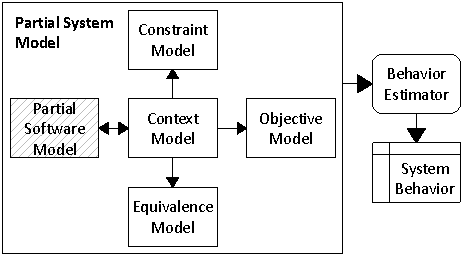
\includegraphics{../gfx/framework.pdf}
	\caption{Overview of the lightweight approach to early traffic flow estimation.}
	\label{fig:framework}
\end{figure}

The approach is similar to work on vehicle path optimization~\cite{Danielsson2007}, which uses Modelica for modeling and Optimica for optimization. However, the author uses continuous-time models instead and concentrates on a single vehicle only.

\section{System Model and Behavior Estimation}

In the following we explain the system model and describe behavior estimation and first estimation results.

\subsubsection*{System Model}

As discussed before, in our system model the traffic infrastructure is represented as directed graph. Nodes constitute reference points in the environment such as intersections and are defined by their absolute position (i.e.\ latitude, longitude and elevation). Edges represent road segments and are defined by source and target node as well as assigned number of lanes. The \textit{context model} is composed of vehicle components, which define several inputs and outputs: Inputs are the speed and the next segment on the traffic infrastructure representing the control decisions. Outputs are the current segment, the distance traveled on the segment, the energy consumption and the state of charge. The energy consumption is estimated from the traveled elevation profile and the speed. Based on the current segments and traveled distances on the segments the \textit{constraint model} tests for collisions. Then, the \textit{objective model} encodes two conflicting objectives: Energy-efficiency and shortest traveling time. Both system-level objectives are decomposed into equivalent vehicle objectives. Per vehicle energy costs are measured in terms of cumulative energy consumption while traveling from origin to destination. In contrast, time costs are measured in terms of time steps needed during the travel. At system-level, the independent vehicle objectives are aggregated using respective weights. To complete the control loop the \textit{software model} encodes \textit{non-deterministic} selection of speed and next segment per vehicle. The speed is selected from a continuous interval ranging from zero to a constant maximum, while the next segments equal to the outgoing segments of the current segment's target node. The \textit{equivalence model} then uses the average state of charge over all vehicles for clustering the state space. This rule has been selected after comparing a few clustering strategies. Finally, a time resolution of 60 seconds is used, i.e.\ the model state is evaluated every 60 seconds.

\subsubsection*{Behavior Estimation}

%As mentioned before, the behavior estimation algorithm is inspired by stochastic approximation techniques~\cite{Pereira1991}.
Starting with the initial system state the behavior estimation algorithm proceeds from time step to time step until a maximum duration is reached. Given the states of the previous time step the algorithm samples a configurable number of states for the current time step by random speed and next segment selection. Then the current states are filtered using the constraint model and clustered using the equivalence model. Subsequently, only the most cost-efficient states per cluster are used. Finally, after the maximum number of time steps the algorithm returns the most cost-efficient state over all clusters. To demonstrate behavior estimation performance, we configured a basic traffic scenario. The scenario includes twenty vehicles, three origins, three destinations, two objectives per vehicle (i.e.\ shortest traveling time and energy-efficiency), and a number of routing options with different distances and elevation profiles. Figure~\ref{figure:graph} shows the traffic infrastructure and the estimated traffic flow for the shortest traveling time objective. Origins and destinations are displayed as triangles. Colored edges represent segments travelled by traffic participants, while dashed edges represent unused segments. The edge thickness corresponds to the number of traffic participants traveling a segment. The edge color depicts traffic participants with same origin and destination. Figure~\ref{figure:chart} finally provides aggregate energy consumption charts for different weights between the time and energy objectives.

%Between origin and destination two different single-laned routes are defined: The first represents a longer, but flat route, while the second describes a shorter, but undulating route. Finally, we analyze two different objective configurations modeled by means of weights: Configuration~A favors lower energy cost, while configuration~B prefers lower time cost. Figure~\ref{figure:results} shows the results of behavior estimation including selected routes (colored by vehicle) and aggregate energy consumption. In the route visualizations edge thickness represents the time steps needed to travel the respective road segments. In configuration~A eight out of ten vehicles decide to take the upper flat route, while overall more time is needed to travel the segments. Instead, in configuration B eight out of ten vehicles decide to take the lower undulating route, while overall less time is needed to travel the segments. These observations are confirmed by the aggregate energy consumption chart: In configuration~A the vehicles require 44\% less energy, but three times as long to travel from origin to destination compared to configuration~B.

\begin{figure}[t!]
	\centering
	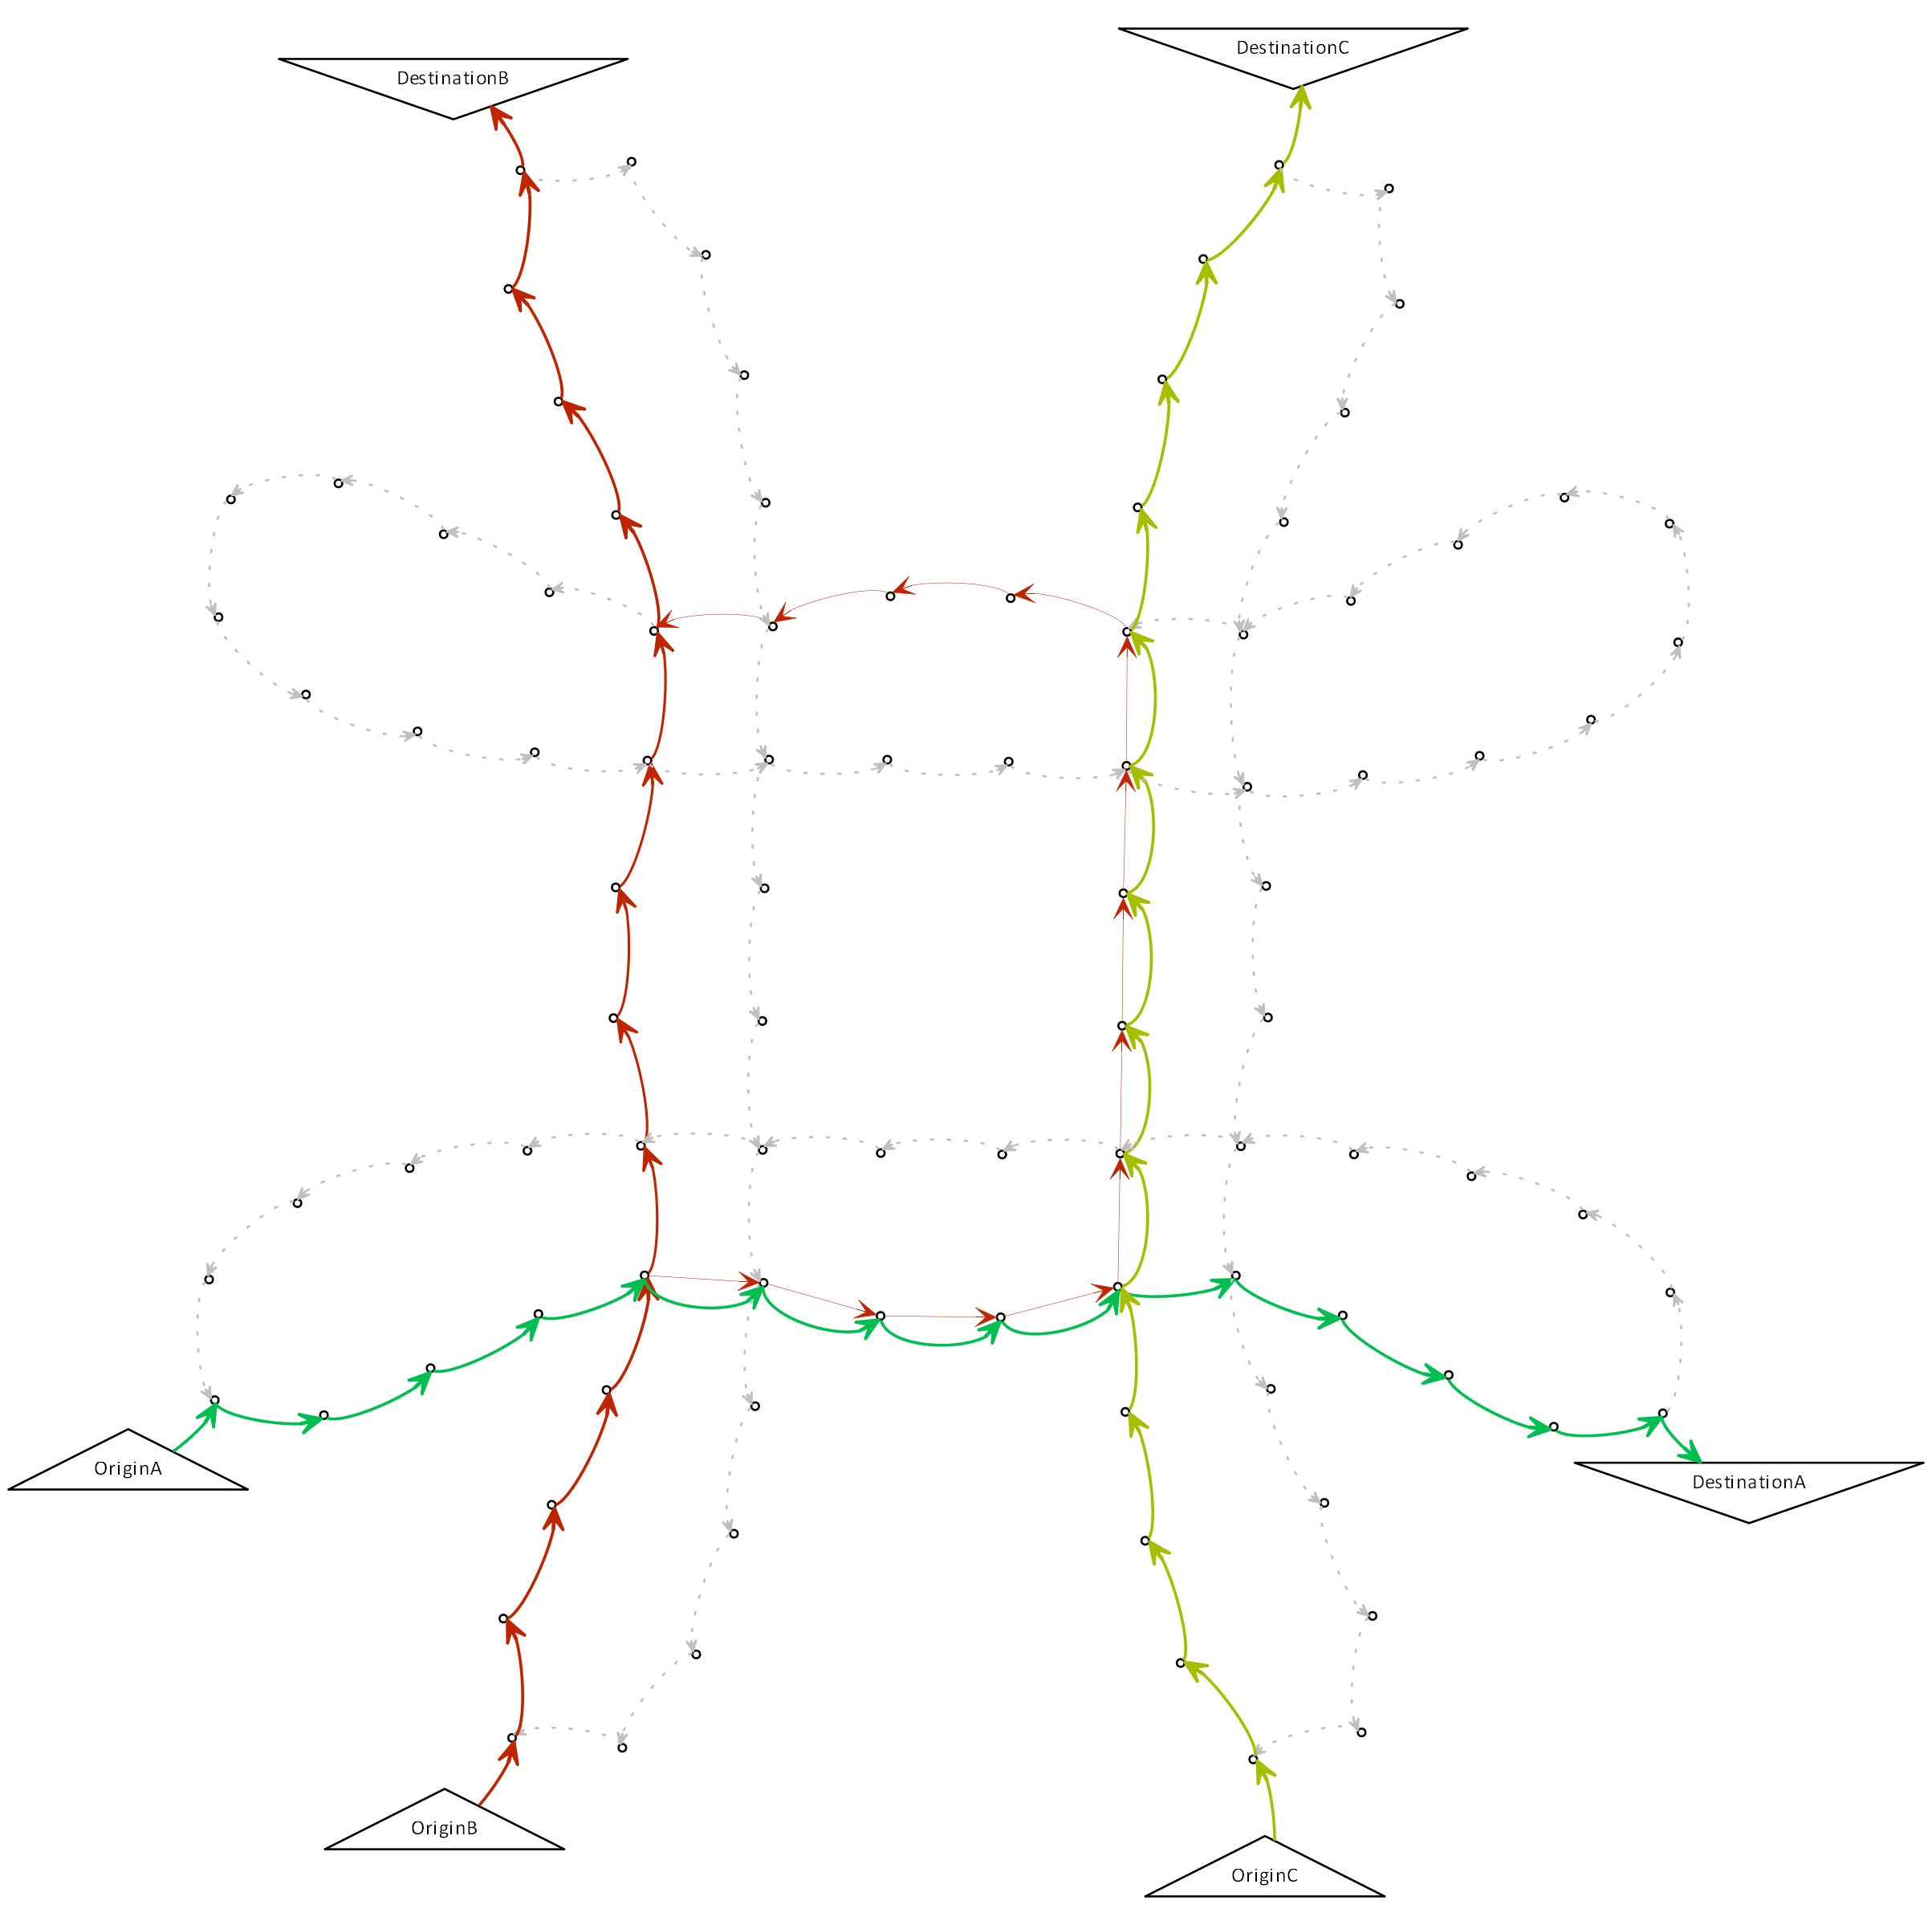
\includegraphics[width=0.925\columnwidth]{../gfx/graph.png}
	\caption{Traffic flow visualization for shortest traveling time objective.}
	\label{figure:graph}
\end{figure}

\begin{figure}[t!]
	\centering
	
\includegraphics[width=0.925\columnwidth]{../gfx/chart.png}
	\caption{Aggregate energy consumption comparison for different objectives.}
	\label{figure:chart}
\end{figure}

\section{Conclusion and Outlook}

The preliminary results are encouraging with respect to the feasibility of the model-based approach for early multi-objective traffic flow estimation. Currently, we are working on vehicle model improvements, more diverse objectives, OpenStreetMap integration and advanced traffic flow estimation strategies to handle larger problem scales efficiently.

\bibliographystyle{../bst/IEEEtran}
\bibliography{ICCVE-2014}

\end{document}
